%!TEX root = ../../novoIndex.tex
\emph{Redes Neurais Convolucionais} (CNNs, do inglês \emph{Convolutional Neural Networks}) são uma classe de redes neurais \emph{feedforward} com topologia bem definida e estrutura em grade, com o uso de operações de convolução em pelo menos uma de suas camadas \cite{goodfellow2016deep}. Aplicadas em tarefas de classificação, regressão, localização, detecção e outras, este tipo de modelo se destaca no reconhecimento de padrões em dados de alta dimensionalidade, a exemplo de séries temporais, imagens e vídeos \cite{Khan:Livro}.

A operação de convolução possui um papel central nas CNNs. Esta operação descreve a média ponderada de uma determinada função $x_1(t)$ sob um intervalo fixo de uma variável, enquanto os pesos da média ponderada considerada pertencem à função $x_2(t)$ amostrados em intervalos $a$ \cite{bracewell1986fourier}. Assim, a convolução $s(t)$ de duas funções $x_1(t)$ e $x_2(t)$ é uma função $s: \mathds{Z} \rightarrow \mathds{R}$, denotada $s(t) = x_1(t) * x_2(t)$, e definida conforme Equação \ref{eq:int_convolucao} \cite{lathi2006sinais}:

\begin{equation}\label{eq:int_convolucao}
s(t) = x_1(t) * x_2(t) = \int_{-\infty}^{\infty} x_1(a) x_2(t-a)da.
\end{equation}

No contexto de ML, a função $x_1(t)$ é chamada de \emph{input}, a função $x_2(t)$ é o \emph{kernel}, e a saída $s(t)$ consiste no \emph{feature map}, ou mapa de características. No contexto prático, o \emph{input} normalmente é um vetor multidimensional de dados e o \emph{kernel} é um vetor multidimensional de pesos que devem ser ajustados para aprendizado das CNNs. Considerando, por exemplo, uma imagem $I$ de dimensões $(m,n)$ como \emph{input} e a aplicação de um \emph{kernel} $K$, a versão discreta da convolução, passível de implementação computacional e equivalente à Equação \ref{eq:int_convolucao}, é mostrada na Equação \ref{eq:conv_img}:
\begin{equation}
 S(i,j) = I(i,j)*K(i,j) = \sum_{m}\sum_{n}I(m,n)K(i-m,j-n),\label{eq:conv_img}
\end{equation}
em que $S$ é o \emph{feature map} resultante e $(i,j)$ é a posição correspondente nesse mapa. Para otimizar os aspectos de implementação, os valores resultantes da operação de convolução são armazenados apenas nas posições $(i,j)$ explicitamente declaradas \cite{goodfellow2016deep}.

Os \emph{feature maps}, resultantes das operações de convolução, compreendem a noção de filtros, responsáveis por capturarem características relativas à entrada, tais como contornos, linhas, texturas, etc. Quando combinados de maneira sequencial, como proposto pelas CNNs, as características capturadas pelas camadas convolucionais vão se tornando mais complexas à medida que se aumenta a profundidade da rede. Assim, um primeiro \emph{feature map} de uma camada convolucional captura um simples contorno, enquanto um \emph{feature map} em uma camada mais profunda da rede pode capturar uma forma, um rosto ou até um objeto inteiro \cite{Buduma:Livro}. Esta noção é ilustrada na Figura \ref{fig:convolutions}.

\begin{figure}[!ht]
	\centering
	\caption{Papel das camadas convolucionais e \emph{feature maps} nas CNNs. Fonte: \cite{Khan:Livro}.}
	\label{fig:convolutions}
	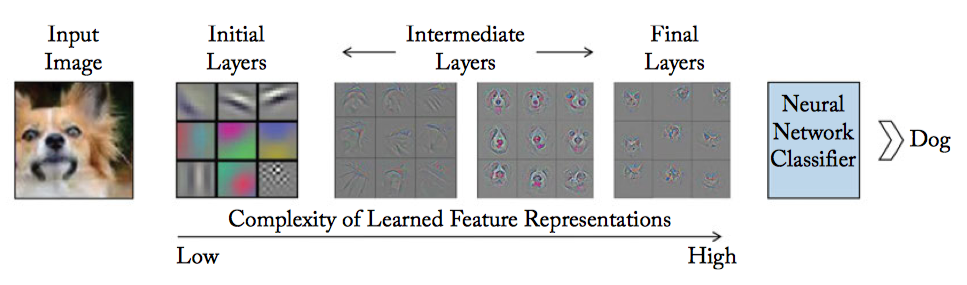
\includegraphics[width=0.8\textwidth]{./img/fundamenta/convolutions}
\end{figure}

As camadas convolucionais, que capturam os \emph{feature maps} e contém os pesos da rede, normalmente são seguidas por funções de ativação como as exemplificadas na Seção \ref{sec:rnas}, mais especificamente na Tabela \ref{tab:ativacoes}. Via de regra, a toda camada convolucional em uma CNN, segue-se uma função de ativação, finalizando em uma operação de \emph{pooling}, como mostra a Figura \ref{fig:cnn_camada}.

\begin{figure}[!ht]
	\centering
	\caption{Componentes de uma camada de uma rede neural convolucional. Adaptado de \cite{goodfellow2016deep}.}
	\label{fig:cnn_camada}
	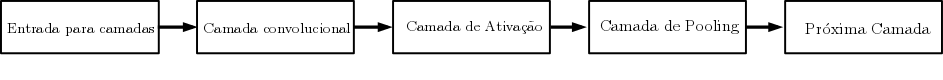
\includegraphics[width=\textwidth]{img/cnn_camada_ipe.png}
\end{figure}

 Uma função de \emph{pooling}, por sua vez, substitui a saída da rede em determinada localização por uma síntese estatística das saídas vizinhas. Por exemplo, a operação \emph{max pooling} retorna o valor máximo em uma área retangular, enquanto a \emph{average pooling} retorna a média das saídas de um retângulo. O objetivo desta operação é fazer com que o \emph{feature map} seja invariante a pequenas mudanças na entrada. Esta invariância a pequenas mudanças locais é uma propriedade útil quando o mais importante for a existência da característica e não exatamente a sua posição, o que aumenta a eficiência geral da CNN ao reduzir drasticamente o número de valores a serem passados entre duas camadas quaisquer \cite{goodfellow2016deep}.

 Outros parâmetros, como \emph{padding} e \emph{strides}, são importantes para a captura de características. O parâmetro \emph{padding} consiste em adicionar um número de linhas e colunas em cada lado da entrada de maneira a controlar o tamanho do \emph{feature map} resultante da operação de convolução. Já a distância entre duas janelas da convolução, ou da operação de \emph{pooling}, é medida através do número de \emph{strides}. Ambos parâmetros manipulam as dimensões das saídas das camadas de uma CNN \cite{chollet2017deep}.

Embora se tenha uma noção clara das camadas individuais e de suas respectivas funções, a combinação das mesmas em uma rede neural convolucional não é uma tarefa trivial, podendo resultar em um número arbitrariamente grande de redes com milhares de parâmetros ajustáveis, cujo desempenho acerca de um problema ainda precisará ser aferido. Considerando os esforços computacionais para isto, a maioria das soluções atuais baseadas em DL fazem uso de CNNs canônicas já propostas na literatura, as quais são apresentadas a seguir.
